\documentclass[12pt]{article}

\usepackage{amsmath}
\usepackage{amsfonts}
\usepackage{graphicx}

\title{CAGD - Abgabe 1: Results} 
\author{Stefan Zaufl \\ Hanna Huber}

\begin{document}
\maketitle

\section{Aufgabe 1}

\begin{figure}
\centering{
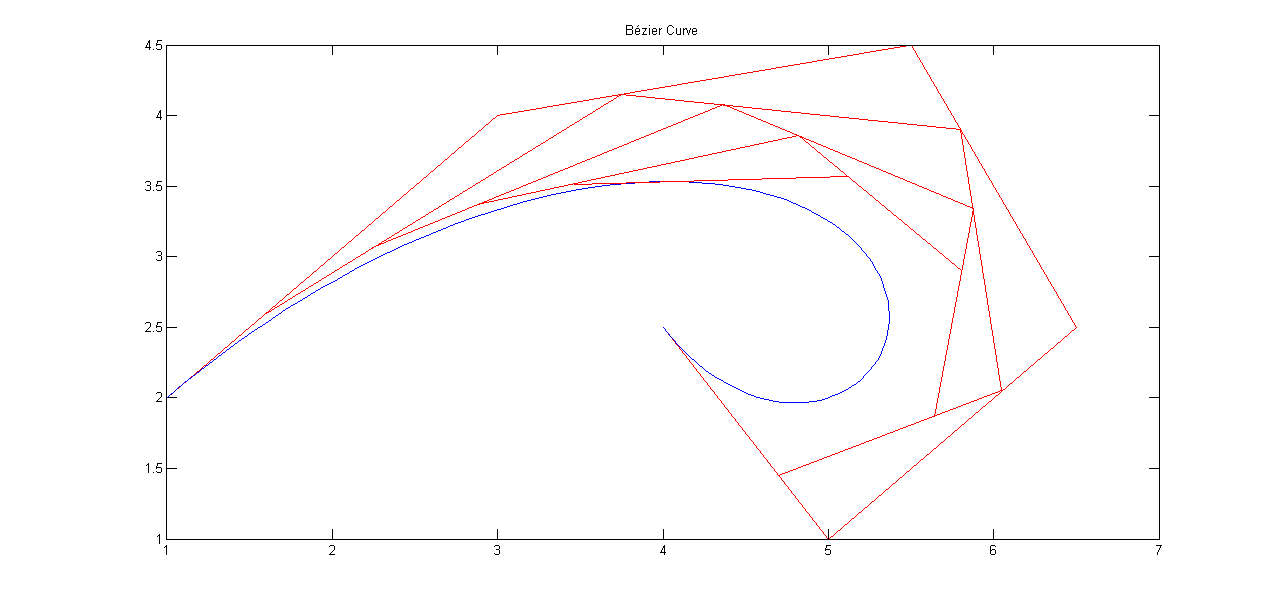
\includegraphics[width=\textwidth]{1a.png}}
\caption{The algorithm of de Casteljau for t=0.3}
\label{fig:1a}
\end{figure}

The algorithm of de Casteljau is illustrated in Figure~\ref{fig:1a}. Figure~\ref{fig:1b} shows that a Bezier curve is well approximated by the control polygon created by consecutively applying the algorithm of the de Casteljau. Note that only three iterations are sufficient to compute a good approximation.

\begin{figure}
\centering{
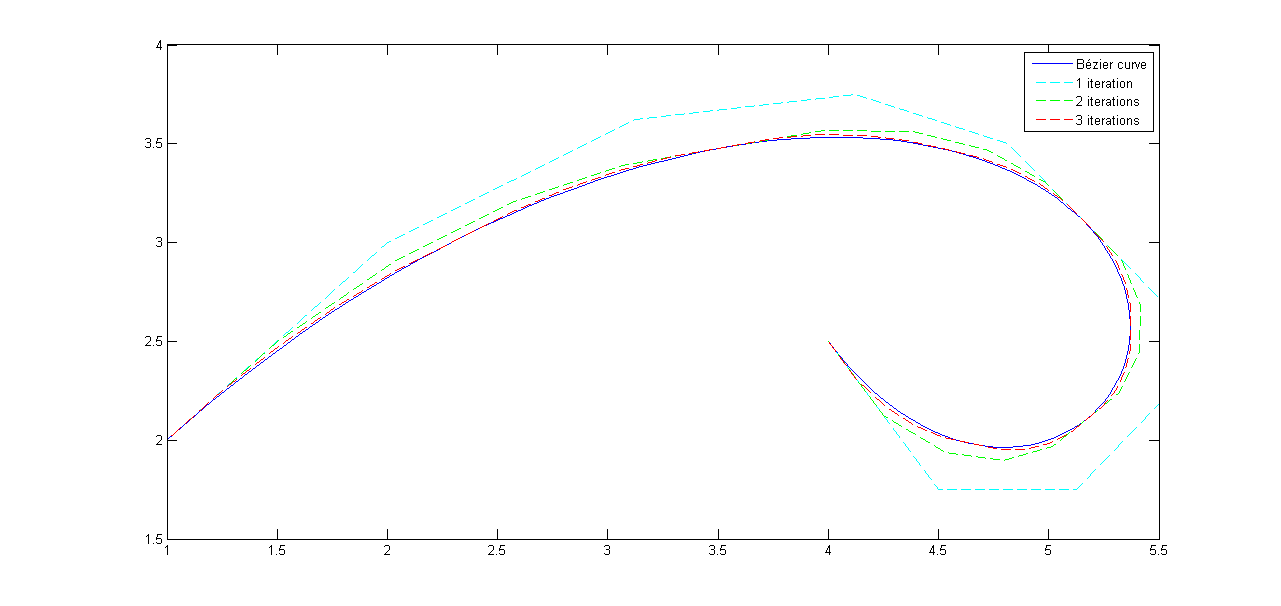
\includegraphics[width=\textwidth]{1b.png}}
\caption{Comparison of the Bezier curve and its approximations applying the algorithm of de Casteljau one, two and three times, respectively.}
\label{fig:1b}
\end{figure}


\section{Aufgabe 2}

\textbf{Proposition.} A Bezier curve $f(t)$ of degree $n$ with control points $P_0, P_1, ... P_n$ can be written as a Bezier curve $g(t)$ of degree $n+1$ with control points $Q_0, Q_1, ... Q_{n+1}$, where 

\begin{eqnarray}
 Q_0 &=& P_0  \label{eq:q0}\\
Q_j &=& \frac{j}{n+1}P_{j-1} + \left(1 - \frac{j}{n+1}\right)P_{j} \label{eq:q}
\end{eqnarray}

\textbf{Proof.} We want to show that $g(t) = f(t)$ for all $t\in R$ if we define the control points $Q_i, i=0...n+1$ as in Equations~\ref{eq:q0} and~\ref{eq:q} (where Equation~\ref{eq:q0} follows from Equation~\ref{eq:q}). Using the parametric representation of the Bezier curve - and writing $B^n_j:= B^n_j(t)$ for easier notation - we write
\begin{eqnarray*}
g(t) &=&  \sum_{j=0}^{n+1} B_j^{n+1}\left(\frac{j}{n+1}P_{j-1} + \left(1 - \frac{j}{n+1}\right)P_{j}\right) \\
      &=&  \sum_{j=0}^{n+1} B_j^{n+1}\frac{j}{n+1}P_{j-1} +\sum_{j=0}^{n+1} B_j^{n+1} \left(1 - \frac{j}{n+1}\right)P_{j}
\end{eqnarray*}
Note that the first and last term of the first and second sum, respectively, equals 0. Therefore we can write 
\begin{eqnarray*}
&&  \sum_{j=0}^{n+1} B_j^{n+1}\frac{j}{n+1}P_{j-1} +\sum_{j=0}^{n+1} B_j^{n+1} \left(1 - \frac{j}{n+1}\right)P_{j} \\
&=&  \sum_{j=1}^{n+1} B_j^{n+1}\frac{j}{n+1}P_{j-1} +\sum_{j=0}^{n} B_j^{n+1} \left(1 - \frac{j}{n+1}\right)P_{j} \\
&=&  \sum_{j=0}^{n} B_{j+1}^{n+1}\frac{j+1}{n+1}P_{j} +\sum_{j=0}^{n} B_j^{n+1} \left(1 - \frac{j}{n+1}\right)P_{j}
\end{eqnarray*}
Recalling that the Bernstein polynomials are given by
\begin{equation*}
B_j^n(t)={n \choose j}t^j(1-t)^{n-j}
\end{equation*}
we can deduce that
\begin{eqnarray*}
B_{j+1}^{n+1}\frac{j+1}{n+1} &=& \frac{(n+1)!}{(j+1)!(n+1)-(j+1))!}t^{j+1}(1-t)^{n+1-(j+1)} \frac{j+1}{n+1} \\
&=& {n \choose j}t^{j+1}(1-t)^{n-j} \\
&=& tB_j^{n} \\
 B_j^{n+1} \left(1 - \frac{j}{n+1}\right) &=& \frac{(n+1)!}{j!(n+1-j)!}t^{j}(1-t)^{n+1-j} \frac{n+1-j}{n+1}\\
&=& {n \choose j}t^{j}(1-t)^{n+1-j} \\
&=&(1- t)B_j^{n}
\end{eqnarray*}
Consequently,
\begin{eqnarray*}
\sum_{j=0}^{n} B_{j+1}^{n+1}\frac{j+1}{n+1}P_{j} +\sum_{j=0}^{n} B_j^{n+1} \left(1 - \frac{j}{n+1}\right)P_{j} &=& \\
&=& \sum_{j=0}^{n} tB_j^{n}P_{j} +\sum_{j=0}^{n}(1- t)B_j^{n} P_{j} \\
&=& t\sum_{j=0}^{n} B_j^{n}P_{j} + (1- t)\sum_{j=0}^{n}B_j^{n} P_{j} \\
&=& \sum_{j=0}^{n} B_j^{n}P_{j} \\
& =& f(t)
\end{eqnarray*}
\hfill$\square$.


\end{document}